\documentclass[11pt]{article}

\usepackage{amsmath,amssymb,amsfonts}
\usepackage{graphicx}
\usepackage{pgfplots}
\usepackage{multicol}
\usepackage{enumitem}

\setlength{\topmargin}{-.5in} \setlength{\textheight}{9.25in}
\setlength{\oddsidemargin}{0in} \setlength{\textwidth}{6.8in}

\pgfplotsset{soldot/.style={color=black,only marks,mark=*},
             holdot/.style={color=black,fill=white,only marks,mark=*},
             compat=1.12}


\begin{document}

\Large

\noindent{\bf Name: \hfill Date: \hfill Exam 4 \hfill Precalculus - Hargus}

\medskip\hrule
\vspace{20pt}

\noindent \textbf{Instructions:} Please \textbf{show all work} on the test paper (partial credit may be awarded for correct work, even if your answer is wrong).

\vspace{10pt}

\begin{enumerate}

\item (4 points) Convert from radians to degrees or from degrees to radians.
\begin{multicols}{2}
\begin{enumerate}[itemsep=30pt]
    \item $\frac{5\pi}{3}$ (radians) =
    \item $120^{\circ} =$
\end{enumerate}
\end{multicols}
\vspace{30pt}


\item (4 points) Evaluate the expression.
\begin{multicols}{2}
\begin{enumerate}[itemsep=60pt]
    \item $\log_{5}{125} = $
    \item $\tan{180^{\circ}} = $
\end{enumerate}
\end{multicols}
\vspace{60pt}


\item (4 points) Write an equation $f(x)$ for the following exponential graph.
\vspace{10pt}
\begin{center}
\begin{tikzpicture}
\begin{axis}[ xlabel={$x$}, ylabel={$y$}
  ,axis lines=middle
  ,height=10cm, width=10cm,
  ,samples=1000, grid, thick
  ,domain=-10:10
  ,restrict y to domain=-10:10
  ,axis equal
  ,legend pos=outer north east
  ,xmin=-5, xmax=5,
  ,ymin=-3, ymax=10
  ]
\addlegendentry{$f(x)$}
\addplot+[no marks] {2.718^(x+1)};
\node[label={45:{$(1,e^2)$}},circle,fill,inner sep=2pt] at (axis cs:1,7.388) {};
\node[label={left:{$(-1,1)$}},circle,fill,inner sep=2pt] at (axis cs:-1,1) {};
\end{axis}
\end{tikzpicture}
\end{center}

\begin{flushright}
$f(x) =$ \rule{4cm}{0.4pt}
\end{flushright}


\newpage



\item (6 points) Solve for x.
\begin{multicols}{2}
\begin{enumerate}[itemsep=50pt]
    \item $\displaystyle \frac{\ln(x)}{e} = e^3$
    \item $\displaystyle \sin(x)=\frac{\sqrt{2}}{2} \hspace{20pt} \left(\frac{\pi}{2} \leq x \leq \pi \right)$
\end{enumerate}
\end{multicols}
\vspace{100pt}


\item (8 points) Consider the function $f(x) = \frac{1}{x-3} + 2$. True or false?
\begin{enumerate}[itemsep=20pt]
    \item \rule{1cm}{0.4pt} $f(x)$ has a horizontal asymptote at $y=3$.
    \item \rule{1cm}{0.4pt} $f(x)$ has a vertical asymptote at $x=3$.
    \item \rule{1cm}{0.4pt} $\displaystyle{\lim_{x \to \infty} f(x) = \infty}$
    \item \rule{1cm}{0.4pt} $\displaystyle{\lim_{x \to 3^+} f(x) = \infty}$
\end{enumerate}
\vspace{20pt}

\item (4 points) Use synthetic division to divide the following (Write your answer in \textbf{fraction form}).

\vspace{10pt}
$\displaystyle{\frac{x^3 - 3x^2 - 2x + 25}{x-3}} $
\vspace{100pt}


\newpage


\item (4 points) The graph of $f(x)=\cos(x)$ is below. Draw $g(x)=2\cos(\frac{1}{2}x)$.
\vspace{4pt}
\begin{center}
\begin{tikzpicture}
\begin{axis}[ xlabel={$x$}, ylabel={$y$}
  ,axis lines=middle
  ,samples=1000, grid, thick
  ,domain=-10:10
  ,restrict y to domain=-10:10
  ,legend pos=outer north east
  ,xmin=-6.4, xmax=6.4,
  ,ymin=-3, ymax=3
  , 
    xtick={
        -6.28318, -3.14159, 
        3.14159, 6.28318
    },
    xticklabels={
        $-2\pi$, $-\pi$, 
        $\pi$, $2\pi$
    }
  ]
\addplot+[no marks] {cos(deg(x))};
\addlegendentry{$f(x)$}
\end{axis}
\end{tikzpicture}
\end{center}


\item (4 points) The graph of $f(x)$ is drawn below. Draw the graph of $f^{-1}(x)$.
\vspace{10pt}
\begin{center}
\begin{tikzpicture}
\begin{axis}[ xlabel={$x$}, ylabel={$y$}
  ,axis lines=middle
  ,samples=1000, grid, thick
  ,domain=-10:10
  ,restrict y to domain=-10:10
  ,axis equal
  ,legend pos=outer north east
  ,xmin=-5, xmax=5,
  ,ymin=-5, ymax=5
  ]
\addplot+[no marks] {ln(x-2)};
\addlegendentry{$f(x)$}
\end{axis}
\end{tikzpicture}
\end{center}


\item (4 points) Simplify the expression to either 1 or -1.

\begin{enumerate}[itemsep=60pt, label={\alph*)}]
    \item $\displaystyle \sec(-x) \cos(x) $
    \item $\displaystyle \frac{1}{2}(-2\cos^2(x) - 2\sin^2(x)) $
\end{enumerate}
\vspace{60pt}

\newpage

\item (6 points) Prove the identity.
\begin{enumerate}[itemsep=150pt, label={\alph*)}]
    \item $\displaystyle \cos(x) = \frac{\cot(x)}{\csc(x)}$
    \item $\displaystyle (\sin(x))(\cos(x)\tan(x) + \cot(x)) = \cos(x) + \sin^2(x)$
\end{enumerate}

\vspace{250pt}

\item (4 points) Find an \textbf{explicit} rule for the $n$th term of the sequence.
\begin{enumerate}[itemsep=30pt, label={\alph*)}]
\item 4, 8, 12, 16, ...
\begin{flushright}
$a_n$= $\rule{3cm}{0.4pt}$
\end{flushright}
\item $a_1 = 5$, $a_{n+1}$ = $3a_{n}$
\begin{flushright}
$a_n$= $\rule{3cm}{0.4pt}$
\end{flushright}
\end{enumerate}

\newpage

\item (6 points) You do not need to simplify your answers for these questions: answers with powers, products, and factorials are okay.
\begin{enumerate}[itemsep=20pt, label={\alph*)}]
\item How many ways are there to select a group of 4 students from a class of 8 students? (order does not matter)
\vspace{40pt}
\begin{flushright}
Ways: $\rule{3cm}{0.4pt}$
\end{flushright}
\item How many unqiue ways are there to rearrange the letters in the name CONNOR? (for instance, CRONON is one way)
\vspace{40pt}
\begin{flushright}
Ways: $\rule{3cm}{0.4pt}$
\end{flushright}
\item If I roll a six-sided die 5 times, what is the probability that we get the sequence 5, 4, 3, 2, 1? (order matters here)
\vspace{40pt}
\begin{flushright}
Probability: $\rule{3cm}{0.4pt}$
\end{flushright}
\end{enumerate}

\vspace{20pt}

\item (4 points) Eliminate the parameter $t$ from the following parametric equations. For your answer, write $y$ in terms of $x$.
$$x = 3 - 3t$$
$$y = 2 + t$$
\vspace{50pt}
\begin{flushright}
$y = \rule{4cm}{0.4pt}$
\end{flushright}

\newpage

\vspace{20pt}

\item (4 points) The graph of $r = 4\cos(2\theta) + 1$ is shown below. What are the lengths of the petals $l_1$ and $l_2$?

\begin{center}
\begin{tikzpicture}
  \draw[thick,->,>=latex] (-3,0)--(3,0) node[above] {$x$};
  \draw[thick,->,>=latex] (0,-3)--(0,3) node[left] {$y$};
  \draw[thick,-,>=latex] (0,0)--(-0.9, -1.5588) node[pos=0.8, right] {$l_2$};
  \draw[thick,-,>=latex] (0,0)--(-1.5,2.598) node[pos=0.7, right] {$l_1$};
  \draw[domain=0:360,scale=.6,samples=500] plot (\x:{4*cos(3*\x)+1});
\end{tikzpicture}
\end{center}

\begin{flushright}
$l_1$= $\rule{3cm}{0.4pt}$
\end{flushright}

\begin{flushright}
$l_2$= $\rule{3cm}{0.4pt}$
\end{flushright}


\item (4 points) Below are the matrices $A$ and $B$.  Find the product $AB$. \textbf{Show how you got each element in the answer matrix without a calculator}:

\[
A=
  \begin{bmatrix}
    1 & -1 & 2 \\
    2 & 1 & 3 \\
  \end{bmatrix} \quad
B=
  \begin{bmatrix}
    1 \\
    3 \\
    1
  \end{bmatrix}
\]

\newpage

\item (5 points) Solve the following system of equations \textbf{using an inverse matrix} (you can use a calculator to find the inverse, but show other work): 
$$ 4x + 7y + 1z = 5 $$
$$ 2x + 3y + 2z = 4 $$
$$ 1x + 7z = 3 $$
\vspace{120pt}
\begin{flushright}
$x = \rule{2cm}{0.4pt}$ \\
$y = \rule{2cm}{0.4pt}$ \\
$z = \rule{2cm}{0.4pt}$
\end{flushright}

\vspace{30pt}
\item (5 points) Draw the graph of the ellipse with equation $\displaystyle \frac{(x-1)^2}{9} +  \frac{y^2}{16} = 1$.

\begin{center}
\begin{tikzpicture}
  \draw[thick,->,>=latex] (-4,0)--(4,0) node[above] {$x$};
  \draw[thick,->,>=latex] (0,-4)--(0,4) node[left] {$y$};
\end{tikzpicture}
\end{center}

\item (4 points) Let $A = (3, 4, 5)$, $B = (1, 2, 3)$, and $C = (1, 1, 1)$. 
\begin{enumerate}[itemsep=10pt, label={\alph*)}]

    \item What is the midpoint between $A$ and $C$?
\vspace{100pt}
\begin{flushright}
Midpoint: $\rule{2cm}{0.4pt}$
\end{flushright}
    \item Find the dot product $\overrightarrow{AB} \cdot \overrightarrow{BC}$.
\vspace{100pt}
\begin{flushright}
$\overrightarrow{AB} \cdot \overrightarrow{BC} = \rule{2cm}{0.4pt}$
\end{flushright}
\end{enumerate}

\vspace{20pt}

\item (4 points) Researchers ask 13 students how many cups of coffee they drink each week and get the data below. Draw a box-and-whisker plot to display this data.
$$0, 0, 0, 1, 5, 5, 7, 7, 8, 10, 11, 15, 21$$

\newpage

\item (12 points) Use the graph of $f(x)$ below to answer the following questions.
\begin{center}
\begin{tikzpicture}[]
\begin{axis}[
  xlabel={$x$}, ylabel={$y$}
  ,axis lines=middle
  ,samples=1000, grid, thick,
  ymin=0, ymax=3, ytick={-5,...,5}, ylabel=$y$,
  xmin=0, xmax=3, xtick={-5,...,5}, xlabel=$x$,
  height=10cm, width=10cm,
]
\addplot[blue, domain=-1:1]{\x + 1};
\addplot[blue, domain=1:2]{-\x + 3};
\addplot[blue, domain=2:5]{2};
 
\addplot[holdot, color=blue, fill=white] coordinates{(2,1)};
\addplot[soldot, color=blue] coordinates{(2,2)};

\end{axis}
\end{tikzpicture} 
\end{center}

\begin{enumerate}[itemsep=10pt, label={\alph*)}]
\item Does $\displaystyle \lim_{x \to 1} f(x)$ exist? If yes, what does it equal?
    \begin{flushright}
$\displaystyle \lim_{x \to 1} f(x) = \rule{2cm}{0.4pt}$ \\
\end{flushright}
\item Does $\displaystyle \lim_{x \to 2^-} f(x)$ exist? If yes, what does it equal?
    \begin{flushright}
$\displaystyle \lim_{x \to 2^-} f(x) = \rule{2cm}{0.4pt}$ \\
\end{flushright}
\item Does $\displaystyle \lim_{x \to 2} f(x)$ exist? If yes, what does it equal?
    \begin{flushright}
$\displaystyle \lim_{x \to 2} f(x) = \rule{2cm}{0.4pt}$ \\
\end{flushright}
    \item Does $f'(0)$ exist? If yes, what does it equal?
    \begin{flushright}
$\displaystyle f'(0) = \rule{2cm}{0.4pt}$ \\
\end{flushright}
    \item Does $f'(1)$ exist? If yes, what does it equal?
    \begin{flushright}
$\displaystyle f'(1) = \rule{2cm}{0.4pt}$ \\
\end{flushright}
    \item Find $\displaystyle \int_{0}^{3} f(x)dx$.
    \begin{flushright}
$\displaystyle \int_{0}^{3} f(x)dx = \rule{2cm}{0.4pt}$ \\
\end{flushright}

\end{enumerate}

\newpage



\vspace{20pt}

\end{enumerate}

\end{document} 


\item (\textbf{Extra Credit:} 5 points) Prove the following statement for all positive integers $n$ using induction. \\
$$8 + 10 + 12 + ... + (2n + 6) = n^2 + 7n$$
